
\فصل{روش پیشنهادی}

فصل حاضر به شرح مراحل عملیاتی پروژه اختصاص دارد.
در این بخش ابتدا نحوه‌ی آماده‌سازی مجموعه‌داده شرح داده می‌شود.
سپس بررسی می‌شود که این تصاویر دستخوش چه تغییراتی شده و چگونه به مدل ورودی داده می‌شوند.
در ادامه، طراحی انجام‌شده برای مدل یادگیری ماشین توصیف می‌شود.
بخش انتهایی این بخش نیز به ذکر 
جزئیات فرایند آموزش مدل و مقدمه‌ای بر فرایند آزمایش مدل خواهد گذشت.

\قسمت{آماده‌سازی مجموعه‌داده}

داده‌هایی که از مراکز پزشکی دریافت می‌شوند، مسیر طولانی‌ای را طی می‌کنند تا برای آموزش مدل قابل استفاده باشند.
اولین مرحله‌ی این آماده‌سازی شامل نگاشت اطلاعات بیماران به تصاویر می‌باشد.
این نگاشت از طریق شماره‌ی شناسه‌ی بیمار صورت می‌گیرد 
و در نتیجه‌ی آن، اطلاعات پزشکی در دسترس از بیماران به همراه مسیر ذخیره‌سازی تصاویر وی به صورت ساخت‌یافته‌ای جمع‌آوری می‌شوند.\

مرحله‌ی بعد، جداسازی تصاویر مورد توجه پژوهش است.
تصویربرداری‌های انجام‌شده از بیماران، معمولا تنها شامل مغز نمی‌شوند و تصاویری از ریه و \dots را نیز در بر دارند.
به علاوه در هر مجموعه، تعداد تصاویر مغزی نیز با مجموعه‌های دیگر می‌تواند تفاوت داشته باشد.
به گونه‌ای که یک بیمار ۱۵ و بیمار دیگر، ۵۰ برش از مغز را در مجموعه‌ی خود داشته باشد.
این در حالی است که در امتیازدهی ASPECT تنها چند برش خاص از مغز مورد استفاده قرار می‌گیرد.
به این ترتیب، یکی از گام‌های ضروری برای آماده‌سازی داده‌ها، جداسازی این برش‌ها از میان تمام 
تصاویر دریافت‌شده از بیماران و تهیه‌ی یک نگاشت مدون از هر بیمار به برش‌های استخراج‌شده از تصاویر وی می‌باشد.\\

با انجام دو اقدام فوق که بیشتر مربوط به مرتب‌سازی و خالص‌سازی اطلاعات بودند، نوبت به مرحله‌ی پیش‌پردازش
\footnote{Preprocessing}
تصاویر می‌رسد.
پیش‌پردازش یکی از مهم‌ترین و موثرترین گام‌های یادگیری ماشین محسوب می‌شود که ارتباط مستقیمی با عملکرد و توانایی یادگیری مدل دارد. 
درواقع پیش‌پردازش شامل تغییراتی در داده‌های ورودی است که باعث می‌شود تا جای ممکن، اطلاعات نامفید از داد‌ه‌ها حذف شوند و اطلاعات کلیدی نیز در قالب مناسبی به مدل عرضه شوند.
به این ترتیب فرایند یادگیری برای مدل ساده‌تر خواهد بود.
نکته‌ی دیگری که باعث اهمیت بیش‌تر پیش‌پردازش می‌شود، قابلیت استفاده‌ی مجدد آن در پژوهش‌های دیگر است.
درواقع گام پیش‌پردازش تصاویر پزشکی در بسیاری از پژوهش با هم اشتراکات زیادی دارد.
روش‌های ارائه شده در این پروژه نیز می‌توانند در پیش‌پردازش تصاویر CT در سایر تحقیقات راهگشا باشند.
در ادامه، فرایند پیش‌پردازش مورد استفاده در این پژوهش، به صورت گام به گام بر روی یک تصویر مغزی انتخابی شرح داده می‌شوند.

\subsection{افزایش وضوح}
همانطور که در بخش مفاهیم اولیه ذکر شد، مقدار عددی هر پیکسل در تصاویر پزشکی، بازه‌ی بزرگی را شامل می‌شود.
این در حالی است که چشم انسان تنها تعداد محدودی رنگ خاکستری را می‌تواند از هم تمیز دهد.
به همین دلیل، در صورت مشاهده‌ی یک تصویر CT خام، جزئیات بافت مغز و حتی ناحیه‌ی آسیب‌دیده، قابل مشاهده نخواهد بود. 
با این توضیح، تصویر انتخابی برای شرح مراحل پیش‌پردازش، در ابتدا مانند 
شکل \ref{fig:raw-ct} است.
\footnote{ناحیه‌ی مغز برای مقاصد نمایشی، کمی جا‌به‌جا شده‌است.}
بنابراین، در اولین گام، لازم است وضوح تصاویر افزایش داده‌شود.\\

\begin{figure}[ht]
\centering
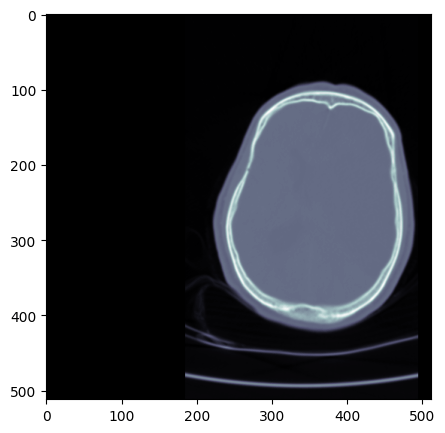
\includegraphics[width=\textwidth, keepaspectratio]{raw-ct.png}
\caption[]{تصویر انتخابی برای نمایش مراحل پیش‌پردازش، در حالت اولیه.}
\label{fig:raw-ct}
\end{figure}

 میان مقدار هر پیکسل با بافت یا شیئی که نمایش می‌دهد ارتباط وجود دارد.
به نحوی که آب، مقدار $0 HU$، هوا مقدار $-1000 HU$، بافت استخوانی مقدار $1000 HU$ و بافت مغزی در حدود $20-50 HU$ می‌باشد.
% Chapter 1 - Computed tomography imaging and angiography – principles
% Author links open overlay panelShervin Kamalian 1, Michael H. Lev 2, Rajiv Gupta 1
به این ترتیب، با محدود کردن مقدار پیکسل‌ها به بازه‌ای مثل $0-100 HU$، اطلاعات مربوط به بافت مغز از بین نمی‌رود.
اما این بار به علت کاهش بازه‌ی رنگ خاکستری، اجزای تصویر از هم بهتر تمایز می‌یابند.
در اصطلاح تصاویر پزشکی، به بازه‌ای که مقادیر به آن محدود می‌شوند پهنای پنجره 
\footnote{Window Width}
و به مرکز این بازه سطح پنجره 
\footnote{Window Level} گفته می‌شود.
با اعمال پهنای پنجره‌ی 100 و سطح پنجره‌ی ۵۰، تصویر اولیه مانند شکل 
\ref{fig:windowed-image}
می‌شود.\\

\begin{figure}[ht]
\centering
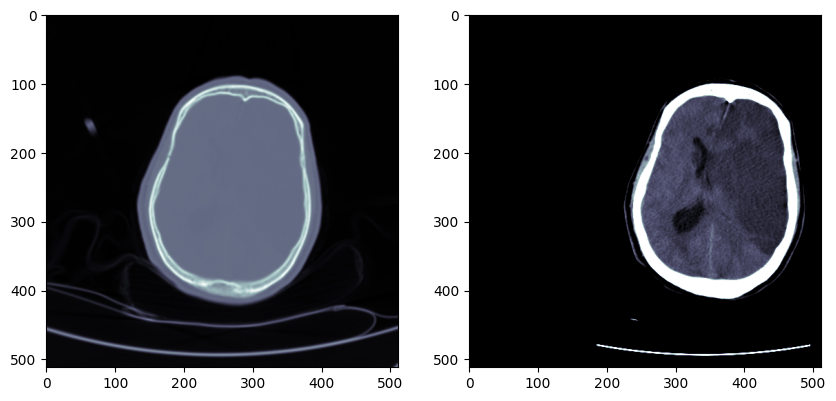
\includegraphics[width=\textwidth, keepaspectratio]{windowed-ct.png}
\caption[]{تصویر انتخابی برای نمایش مراحل پیش‌پردازش، پیش و پس از تنظیم پهنای پنجره به 100 و سطح پنجره به ۵۰. سمت راست، تصویر پس از تنظیم پنجره را نمایش می‌دهد.}
\label{fig:windowed-ct}
\end{figure}

روش معمول برای افزایش وضوح تصاویر، به همین صورت با تنظیم پهنا و سطح پنجره می‌باشد.
اما باید توجه داشت که میان تصاویر بیماران مختلف، تفاوت‌های جزئی وجود دارد.
برخی تصاویر ممکن است به طور کلی قدری تیره‌تر و یا روشن‌تر باشند.
در نتیجه اعمال یک سیاست واحد برای پهنا و سطح پنجره ممکن است برای تمام تصاویر، بهینه نباشد و وضوح لازم را برای تصویر فراهم نکند.
در این پژوهش، از یک روش پویا برای تنظیم وضوح تصاویر استفاده شده‌است که شرح آن در ادامه می‌آید.\\

در این روش، ابتدا مقدار پیکسل‌های مربوط به بافت مغزی هر بیمار به صورت یک مجموعه، استخراج می‌شوند.
سپس چند درصد پایین و چند درصد بالای این مقادیر محاسبه می‌شوند.
در نتیجه، یک چندک
\footnote{quantile} 
پایین و یک چندک بالا به‌دست می‌آید.
در نهایت، مقادیر پیکسل‌های کل تصویر، محدود به بازه‌ی میان این دو چندک می‌شوند.
به این ترتیب، در هر تصویری، با توجه به اطلاعات آماری همان تصویر، 
مقدار پیکسل‌ها محدود به بازه‌ای از رنگ خاکستری می‌شود که اطلاعات بیش‌تری در خود دارد.
اعمال این روش پویا، نیازمند استخراج بافت مغزی است که در مراحل انتهایی پیش‌پردازش به‌دست می‌آید.
به همین جهت، از آوردن تصویر آن در این بخش صرف نظر می‌شود
اما تصویر نهایی فرایند پیش‌پردازش، نمایانگر افزایش بیشتر وضوح 
تصاویر نسبت به روش‌های ایستا (مانند تصویر \ref{fig:windowed-ct}) می‌باشد.\\

\subsection{کاهش نویز}

تصاویر اخذ شده از بیماران معمولا دارای نویز هستند.
گاهی این نویز بسیار شدید است و گاهی جزئی بوده و تشخیص آن در نگاه کلی مشکل است.
در این پژوهش، تصاویری که دارای نویز شدید بودند، از مجموعه‌داده حذف شده‌اند.
اما در مورد سایر تصاویر، همچنان نویز اندکی باقی می‌ماند.
در فرایند پیش‌پردازش پیشنهادی، این نویز با دو مرتبه اعمال فیلتر میانه
\footnote{Median Filtering}
در تصاویر، کاهش می‌یابد.\\

فیلتر میانه به این صورت عمل می‌کند که مقدار هر پیکسل را 
با میانه‌ی پیکسل‌های مجاورش در یک همسایگی مشخص جایگزین می‌کند.
به این ترتیب، اگر تعداد اندکی پیکسل در آن همسایگی، مقادیر پرتی داشته باشند، با مقادیری در محدوده‌ی مناسب، ترمیم می‌شوند.
شدت کاهش نویز به اندازه‌ی همسایگی مورد بررسی در فیلتر میانه بستگی دارد.
هر چه این پنجره بزرگ‌تر باشد، تصویر خروجی محو‌تر و در هم تنیده‌تر
می‌شود.
در مقابل، هر چه فیلتر کوچک‌تر باشد، توانایی کاهش نویزش هم به جمعیت کوچک‌تری محدود می‌شود و برای رفع نویز‌های سنگین مناسب نخواهد بود.
همچنین لازم به ذکر است، یک مزیت فیلتر میانه در آن است که لبه‌های تصویر را بهتر حفظ می‌کند.
بنابراین این فیلتر نسبت به سایر فیلتر‌های کاهش نویز، مانند فیلتر گاوسی، که در برخی کارهای مشابه مورد استفاده قرار می‌گیرند، از این جهت بهتر عمل می‌کند.\\

همانطور که پیش‌تر ذکر شد، در پیش‌پردازش پیشنهادی در این پژوهش، فیلتر میانه دو مرتبه اعمال می‌شود. 
یک مرتبه با پنجره‌ای با اندازه‌ی $7times7$ پیکسل و یک مرتبه با اندازه‌ی $3\times3$ پیکسل.
این مقادیر با آزمون و خطا بر روی تصاویر به‌دست آمده‌اند اما به صورت شهودی نیز می‌توان گفت که به منظور کاهش هر چه بیشتر نویز، دو مرتبه فیلتر نسبتا کوچک اعمال می‌شود.
بار اول برای رفع نویز‌های سنگین‌تر و بار دوم برای بهبود جزئی در یک همسایگی کوچک انجام می شود.
نمونه‌ی کاهش نویز به این روش بر روی تصویر انتخابی 
در شکل
\ref{fig:denoised-ct}
آمده‌است.
البته باید توجه داشت که بهبود تصاویر پس از اعمال فیلتر، در این ابعاد کوچک فیلتر، به سادگی قابل تشخیص نیست.

\begin{figure}[ht]
\centering
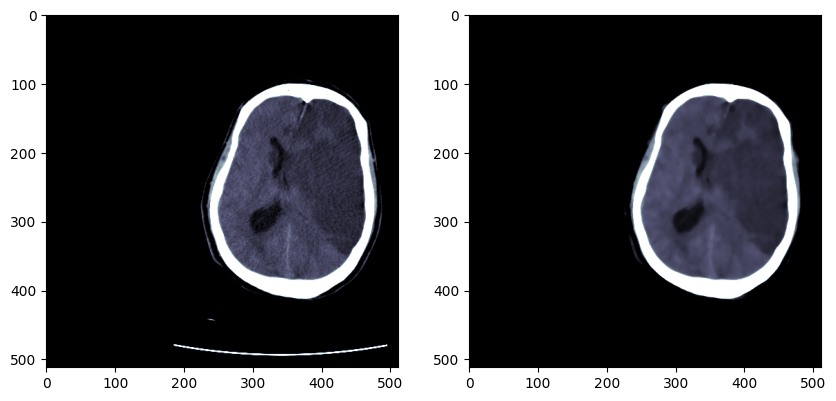
\includegraphics[width=\textwidth, keepaspectratio]{denoised-ct.png}
\caption[]{تصویر انتخابی برای نمایش مراحل پیش‌پردازش، پیش و پس از اعمال فیلتر میانه. سمت راست تصویر پس از اعمال فیلتر را نشان می‌دهد.}
\label{fig:denoised-ct}
\end{figure}
    
\subsection{تنظیم زاویه}
تصاویر مغز ممکن است به دلایلی چون حرکت سر بیمار، همگی زاویه‌ی یکسانی نداشته باشند.
به منظور یک‌دست سازی تصاویر از این جهت، ابتدا ناحیه‌ی سر به صورت یک بیضی تخمین زده می‌شود و سپس با دوران حول یکی از قطر‌هایش، در زاویه‌ی قائم قرار می‌گیرد.
نمونه‌ی این محاسبات و تغییرات در تصویر انتخابی در شکل \ref{fig:aligned-ct}
قابل مشاهده است.

\begin{figure}[ht]
\centering
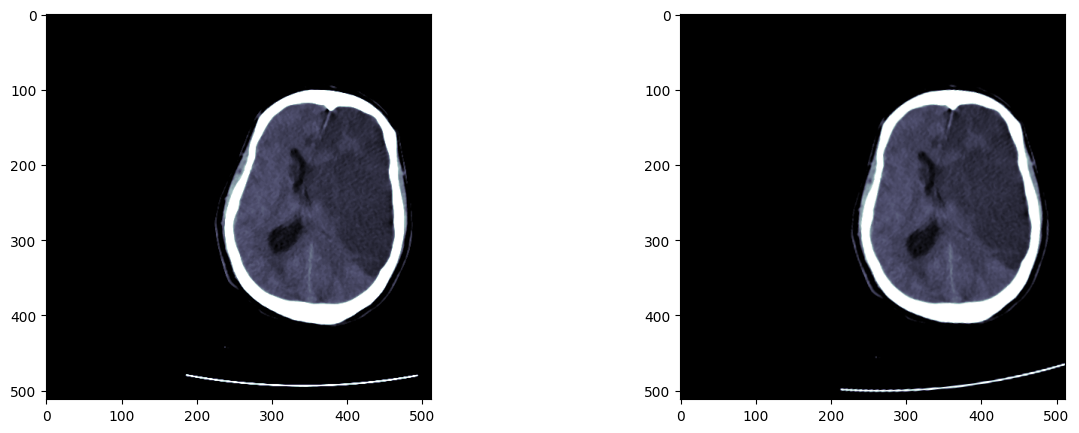
\includegraphics[width=\textwidth, keepaspectratio]{aligned-ct.png}
\caption[]{تصویر انتخابی برای نمایش مراحل پیش‌پردازش، پیش و پس از تنظیم زاویه. سمت راست تصویر پس از تنظیم زاویه را نشان می‌دهد.}
\label{fig:aligned-ct}
\end{figure}

